\section{Question 1}

\textit{\textbf{AIM: Calculate the energy storage capacity Scotland would need to satisfy all its electricity needs with renewable generation and provide a stable grid.}}

According to Scottish Government's quote in assignment description, Scotland's typical electricity demand is 15-16 GW.
\hl{Is this the current typical electricity demand?}

As of Q3 2018, the total installed capacity of renewable energy in Scotland is $10,475 MW$ (see Figure \ref{fig:installed_capacity}), i.e. almost $10.5 GW$ which is two-thirds of Scotland's electricity demand.
\hl{QUESTION: Is all of this RE electricity or is some heat?}
Scotland will thus need to install another $5-6 GW$ of renewable energy capacity to meet the demand.

\hl{QUESTION: Energy capacity = energy storage? Does storage change between renewable technologies?}

\begin{figure}[htbp]
	\centering
	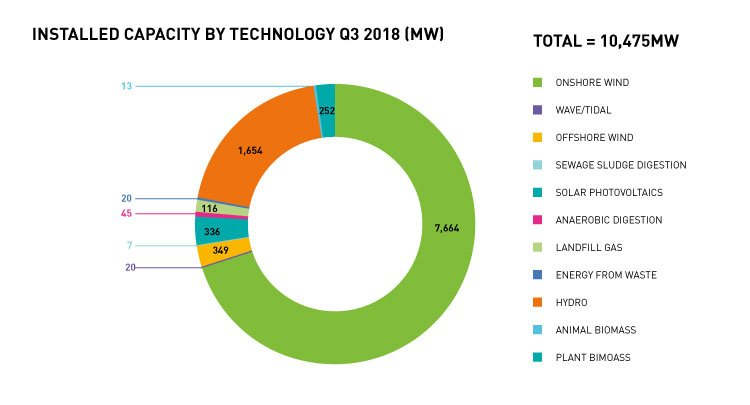
\includegraphics[width=\textwidth]{figures/installed-capacity-by-technology-q3-2018.jpg}
	\rule{\textwidth}{0.5pt} % use line???
	\caption{The installed capacity of renewable energy in Scotland as of Q3 2018 \citep{ScottishRenewables}.}
	\label{fig:installed_capacity}
\end{figure}

